\documentclass[11pt,preprint, authoryear]{elsarticle}

\usepackage{lmodern}
%%%% My spacing
\usepackage{setspace}
\setstretch{1.2}
\DeclareMathSizes{12}{14}{10}{10}

% Wrap around which gives all figures included the [H] command, or places it "here". This can be tedious to code in Rmarkdown.
\usepackage{float}
\let\origfigure\figure
\let\endorigfigure\endfigure
\renewenvironment{figure}[1][2] {
    \expandafter\origfigure\expandafter[H]
} {
    \endorigfigure
}

\let\origtable\table
\let\endorigtable\endtable
\renewenvironment{table}[1][2] {
    \expandafter\origtable\expandafter[H]
} {
    \endorigtable
}


\usepackage{ifxetex,ifluatex}
\usepackage{fixltx2e} % provides \textsubscript
\ifnum 0\ifxetex 1\fi\ifluatex 1\fi=0 % if pdftex
  \usepackage[T1]{fontenc}
  \usepackage[utf8]{inputenc}
\else % if luatex or xelatex
  \ifxetex
    \usepackage{mathspec}
    \usepackage{xltxtra,xunicode}
  \else
    \usepackage{fontspec}
  \fi
  \defaultfontfeatures{Mapping=tex-text,Scale=MatchLowercase}
  \newcommand{\euro}{€}
\fi

\usepackage{amssymb, amsmath, amsthm, amsfonts}

\def\bibsection{\section*{References}} %%% Make "References" appear before bibliography


\usepackage[round]{natbib}

\usepackage{longtable}
\usepackage[margin=2.3cm,bottom=2cm,top=2.5cm, includefoot]{geometry}
\usepackage{fancyhdr}
\usepackage[bottom, hang, flushmargin]{footmisc}
\usepackage{graphicx}
\numberwithin{equation}{section}
\numberwithin{figure}{section}
\numberwithin{table}{section}
\setlength{\parindent}{0cm}
\setlength{\parskip}{1.3ex plus 0.5ex minus 0.3ex}
\usepackage{textcomp}
\renewcommand{\headrulewidth}{0.2pt}
\renewcommand{\footrulewidth}{0.3pt}

\usepackage{array}
\newcolumntype{x}[1]{>{\centering\arraybackslash\hspace{0pt}}p{#1}}

%%%%  Remove the "preprint submitted to" part. Don't worry about this either, it just looks better without it:
\makeatletter
\def\ps@pprintTitle{%
  \let\@oddhead\@empty
  \let\@evenhead\@empty
  \let\@oddfoot\@empty
  \let\@evenfoot\@oddfoot
}
\makeatother

 \def\tightlist{} % This allows for subbullets!

\usepackage{hyperref}
\hypersetup{breaklinks=true,
            bookmarks=true,
            colorlinks=true,
            citecolor=blue,
            urlcolor=blue,
            linkcolor=blue,
            pdfborder={0 0 0}}


% The following packages allow huxtable to work:
\usepackage{siunitx}
\usepackage{multirow}
\usepackage{hhline}
\usepackage{calc}
\usepackage{tabularx}
\usepackage{booktabs}
\usepackage{caption}


\newenvironment{columns}[1][]{}{}

\newenvironment{column}[1]{\begin{minipage}{#1}\ignorespaces}{%
\end{minipage}
\ifhmode\unskip\fi
\aftergroup\useignorespacesandallpars}

\def\useignorespacesandallpars#1\ignorespaces\fi{%
#1\fi\ignorespacesandallpars}

\makeatletter
\def\ignorespacesandallpars{%
  \@ifnextchar\par
    {\expandafter\ignorespacesandallpars\@gobble}%
    {}%
}
\makeatother

\newenvironment{CSLReferences}[2]{%
}

\urlstyle{same}  % don't use monospace font for urls
\setlength{\parindent}{0pt}
\setlength{\parskip}{6pt plus 2pt minus 1pt}
\setlength{\emergencystretch}{3em}  % prevent overfull lines
\setcounter{secnumdepth}{5}

%%% Use protect on footnotes to avoid problems with footnotes in titles
\let\rmarkdownfootnote\footnote%
\def\footnote{\protect\rmarkdownfootnote}
\IfFileExists{upquote.sty}{\usepackage{upquote}}{}

%%% Include extra packages specified by user

%%% Hard setting column skips for reports - this ensures greater consistency and control over the length settings in the document.
%% page layout
%% paragraphs
\setlength{\baselineskip}{12pt plus 0pt minus 0pt}
\setlength{\parskip}{12pt plus 0pt minus 0pt}
\setlength{\parindent}{0pt plus 0pt minus 0pt}
%% floats
\setlength{\floatsep}{12pt plus 0 pt minus 0pt}
\setlength{\textfloatsep}{20pt plus 0pt minus 0pt}
\setlength{\intextsep}{14pt plus 0pt minus 0pt}
\setlength{\dbltextfloatsep}{20pt plus 0pt minus 0pt}
\setlength{\dblfloatsep}{14pt plus 0pt minus 0pt}
%% maths
\setlength{\abovedisplayskip}{12pt plus 0pt minus 0pt}
\setlength{\belowdisplayskip}{12pt plus 0pt minus 0pt}
%% lists
\setlength{\topsep}{10pt plus 0pt minus 0pt}
\setlength{\partopsep}{3pt plus 0pt minus 0pt}
\setlength{\itemsep}{5pt plus 0pt minus 0pt}
\setlength{\labelsep}{8mm plus 0mm minus 0mm}
\setlength{\parsep}{\the\parskip}
\setlength{\listparindent}{\the\parindent}
%% verbatim
\setlength{\fboxsep}{5pt plus 0pt minus 0pt}



\begin{document}



\begin{frontmatter}  %

\title{Russia - Ukraine Conflict}

% Set to FALSE if wanting to remove title (for submission)




\author[Add1]{Nico Katzke\footnote{\textbf{Contributions:}
  \newline \emph{The authors would like to thank the World Happiness
  survey for showing us what happiness is.}}}
\ead{nfkatzke@gmail.com}





\address[Add1]{Satrix, Cape Town}

\cortext[cor]{Corresponding author: Nico Katzke\footnote{\textbf{Contributions:}
  \newline \emph{The authors would like to thank the World Happiness
  survey for showing us what happiness is.}}}

\begin{abstract}
\small{
This article aims to discuss what makes us happy. This is a suggested
solution to question 1.
}
\end{abstract}

\vspace{1cm}





\vspace{0.5cm}

\end{frontmatter}

\setcounter{footnote}{0}



%________________________
% Header and Footers
%%%%%%%%%%%%%%%%%%%%%%%%%%%%%%%%%
\pagestyle{fancy}
\chead{}
\rhead{}
\lfoot{}
\rfoot{\footnotesize Page \thepage}
\lhead{}
%\rfoot{\footnotesize Page \thepage } % "e.g. Page 2"
\cfoot{}

%\setlength\headheight{30pt}
%%%%%%%%%%%%%%%%%%%%%%%%%%%%%%%%%
%________________________

\headsep 35pt % So that header does not go over title




\begin{Shaded}
\begin{Highlighting}[]
\FunctionTok{rm}\NormalTok{(}\AttributeTok{list =} \FunctionTok{ls}\NormalTok{()) }\CommentTok{\# Clean your environment:}
\FunctionTok{gc}\NormalTok{() }\CommentTok{\# garbage collection {-} It can be useful to call gc after a large object has been removed, as this may prompt R to return memory to the operating system.}
\end{Highlighting}
\end{Shaded}

\begin{verbatim}
##          used (Mb) gc trigger (Mb) max used (Mb)
## Ncells 473810 25.4    1023550 54.7   660385 35.3
## Vcells 879837  6.8    8388608 64.0  1770048 13.6
\end{verbatim}

\begin{Shaded}
\begin{Highlighting}[]
\FunctionTok{library}\NormalTok{(tidyverse)}
\end{Highlighting}
\end{Shaded}

\begin{verbatim}
## Warning: package 'tidyverse' was built under R version 4.3.3
\end{verbatim}

\begin{verbatim}
## Warning: package 'ggplot2' was built under R version 4.3.3
\end{verbatim}

\begin{verbatim}
## Warning: package 'lubridate' was built under R version 4.3.3
\end{verbatim}

\begin{verbatim}
## -- Attaching core tidyverse packages ------------------------ tidyverse 2.0.0 --
## v dplyr     1.1.4     v readr     2.1.5
## v forcats   1.0.0     v stringr   1.5.1
## v ggplot2   3.5.0     v tibble    3.2.1
## v lubridate 1.9.3     v tidyr     1.3.1
## v purrr     1.0.2     
## -- Conflicts ------------------------------------------ tidyverse_conflicts() --
## x dplyr::filter() masks stats::filter()
## x dplyr::lag()    masks stats::lag()
## i Use the conflicted package (<http://conflicted.r-lib.org/>) to force all conflicts to become errors
\end{verbatim}

\begin{Shaded}
\begin{Highlighting}[]
\FunctionTok{source}\NormalTok{(}\StringTok{"code/process\_data.R"}\NormalTok{)}
\FunctionTok{list.files}\NormalTok{(}\StringTok{\textquotesingle{}code/\textquotesingle{}}\NormalTok{, }\AttributeTok{full.names =}\NormalTok{ T, }\AttributeTok{recursive =}\NormalTok{ T) }\SpecialCharTok{\%\textgreater{}\%}\NormalTok{ .[}\FunctionTok{grepl}\NormalTok{(}\StringTok{\textquotesingle{}.R\textquotesingle{}}\NormalTok{, .)] }\SpecialCharTok{\%\textgreater{}\%} \FunctionTok{as.list}\NormalTok{() }\SpecialCharTok{\%\textgreater{}\%} \FunctionTok{walk}\NormalTok{(}\SpecialCharTok{\textasciitilde{}}\FunctionTok{source}\NormalTok{(.))}
\end{Highlighting}
\end{Shaded}

\begin{Shaded}
\begin{Highlighting}[]
\CommentTok{\#Loading in the data}
\NormalTok{alloc }\OtherTok{\textless{}{-}} \FunctionTok{read\_csv}\NormalTok{(}\StringTok{"data/Financial Allocations.csv"}\NormalTok{)}
\end{Highlighting}
\end{Shaded}

\begin{verbatim}
## Rows: 41 Columns: 7
## -- Column specification --------------------------------------------------------
## Delimiter: ","
## chr (1): Country
## dbl (6): EU member, Financial allocations($ billion), Humanitarian allocatio...
## 
## i Use `spec()` to retrieve the full column specification for this data.
## i Specify the column types or set `show_col_types = FALSE` to quiet this message.
\end{verbatim}

\begin{Shaded}
\begin{Highlighting}[]
\NormalTok{commit }\OtherTok{\textless{}{-}} \FunctionTok{read\_csv}\NormalTok{(}\StringTok{"data/Financial Commitments.csv"}\NormalTok{)}
\end{Highlighting}
\end{Shaded}

\begin{verbatim}
## Rows: 42 Columns: 11
## -- Column specification --------------------------------------------------------
## Delimiter: ","
## chr  (1): Country
## dbl (10): EU member, GDP in 2021($ billion), Financial commitments($ billion...
## 
## i Use `spec()` to retrieve the full column specification for this data.
## i Specify the column types or set `show_col_types = FALSE` to quiet this message.
\end{verbatim}

\#Question 3

Graphs have been constructed to see how the EU members compares to other
countries with respect to giving aid to Ukraine to help alleviate the
burden of war.

Below aid allocation and aid comitmment has been graphed as well as, and
the reason that aid was given

\begin{Shaded}
\begin{Highlighting}[]
\NormalTok{alloc\_plus\_commit }\OtherTok{\textless{}{-}} \FunctionTok{process\_data}\NormalTok{(alloc, commit)}
\end{Highlighting}
\end{Shaded}

\begin{verbatim}
## Warning: package 'janitor' was built under R version 4.3.3
\end{verbatim}

\begin{verbatim}
## 
## Attaching package: 'janitor'
\end{verbatim}

\begin{verbatim}
## The following objects are masked from 'package:stats':
## 
##     chisq.test, fisher.test
\end{verbatim}

\begin{Shaded}
\begin{Highlighting}[]
\FunctionTok{plot\_allocation\_data}\NormalTok{(alloc\_plus\_commit)}
\end{Highlighting}
\end{Shaded}

\begin{verbatim}
## Warning: Removed 3 rows containing missing values or values outside the scale range
## (`geom_bar()`).
\end{verbatim}

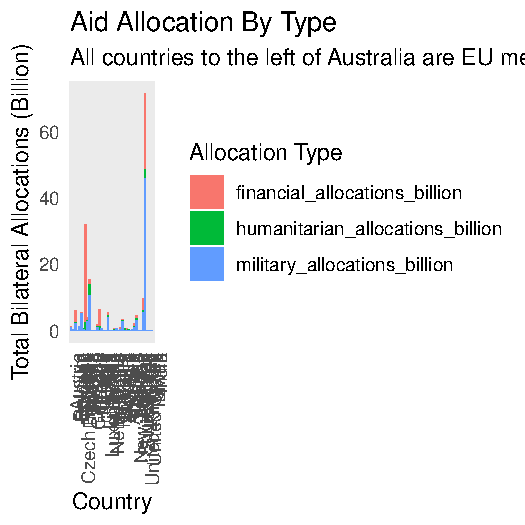
\includegraphics{Question_3_files/figure-latex/unnamed-chunk-3-1.pdf}
From the above graph one can see that aid allocation from the UK far
outweighs allocation from EU Members. It is also interesting to note
that the UK has committed quite a bit of military aid whereas If one
looks to the EU. Those countries commit more to financial allocations

\begin{Shaded}
\begin{Highlighting}[]
\FunctionTok{plot\_commitment\_data}\NormalTok{(alloc\_plus\_commit)}
\end{Highlighting}
\end{Shaded}

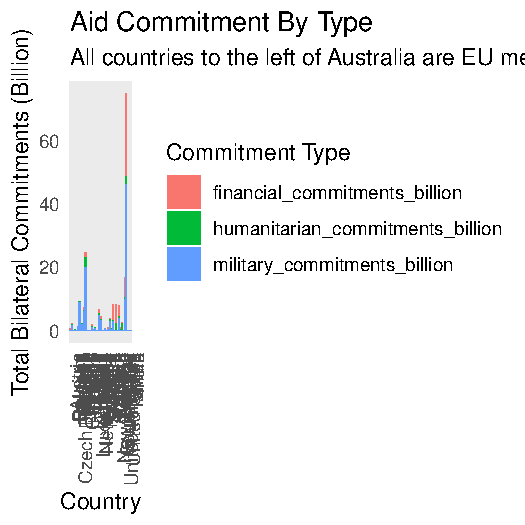
\includegraphics{Question_3_files/figure-latex/unnamed-chunk-4-1.pdf}
The same pattern is seen for commitment. This graphic shows that the EU
could be doing more when coming to aid Ukraine in the face of war

\bibliography{Tex/ref}





\end{document}
